\documentclass[main.tex]{subfiles}
\begin{document}
处理字的符的 Python 程序

\begin{figure}
	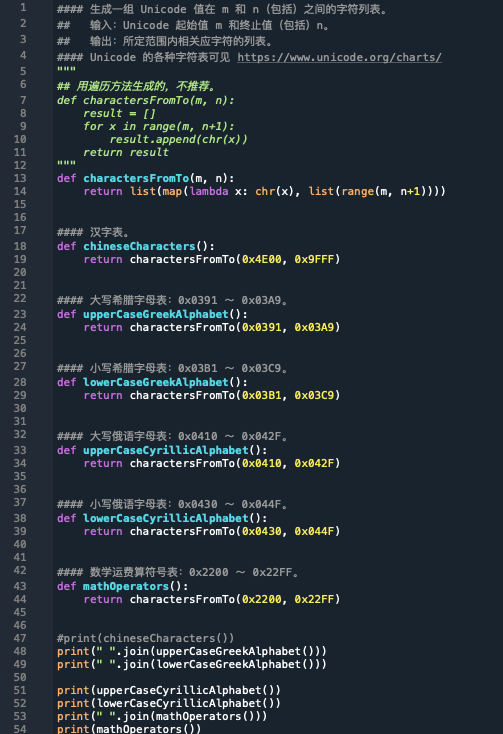
\includegraphics[viewport=0 0 490 735, clip]{png/string.png}
\end{figure}

Python 程序 xxx 生成希腊的字母如下:


从 Unicode 表中 Python 程序 xxx 生成部分常用数学运算速度符号如果下:


\begin{figure}
	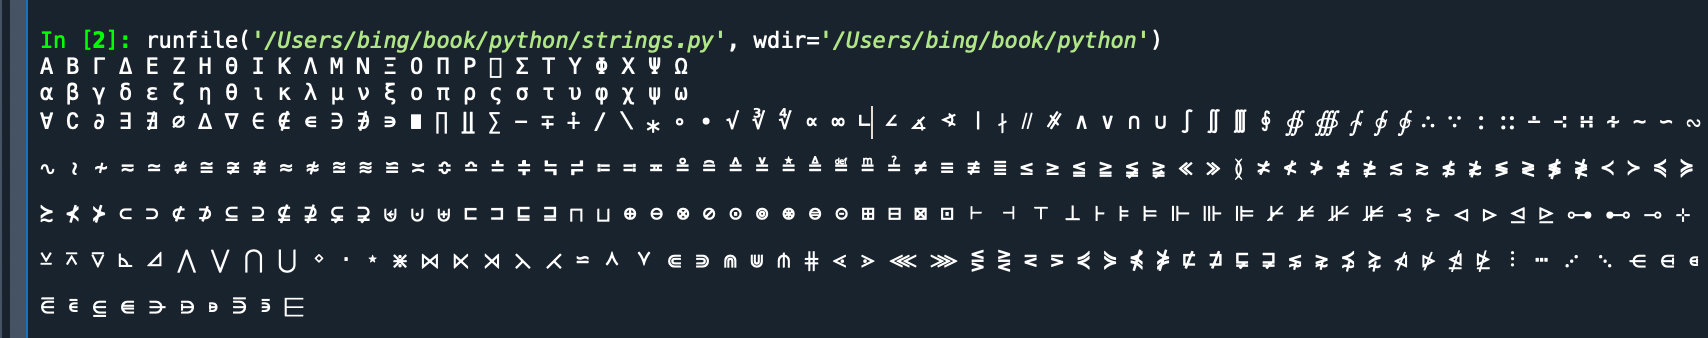
\includegraphics[viewport=0 0 490 200, clip]{png/greek_math_symbols.png}
\end{figure}


字符串处理

\begin{Exercises}
	\item 把下列值代入函数 \verb|int()| 后的结果是什么?

	\begin{tabular}{l l l l} 
	(a) 4.5; & (b) 4.4;  & (c) -4.5; & (d) -4.4; \\
	(e) \verb|True|;  & (f) \verb|False|; & (g) \verb|true|;  & (h) \verb|false|; \\
	(i) 5 == 1+4;  & (j) 6 < 5; & (k) 6 > -1.2; & (l) \textsf{'}3.14159\textsf{'}; \\
	\end{tabular}
	\item 把下列各对值代入函数 \verb|int()| 后的结果是什么?

\begin{tabular}{l l l l} 
	(a) 4.5; & (b) 4.4;  & (c) -4.5; & (d) -4.4; \\
	(e) \verb|True|;  & (f) \verb|False|; & (g) \verb|true|;  & (h) \verb|false|; \\
	(i) 5 == 1+4;  & (j) 6 < 5; & (k) 6 > -1.2; & (l) \textsf{'}3.14159\textsf{'}; \\
\end{tabular}

\end{Exercises}

\end{document} 